\documentclass[xcolor=dvipsnames,mathserif,12pt,backend=biber]{beamer}
\usepackage{graphicx}
\usepackage{tikz}
\usepackage{url}
\usepackage{biblatex}
\usepackage{tabularx}
\usepackage{multirow}
\usepackage{amsmath}
\usepackage{listings}
\usepackage[OT4]{fontenc}
\usepackage[T1]{fontenc}
\usecolortheme[named=Plum]{structure} 
\usetheme[height=10mm]{Rochester} 
\setbeamertemplate{navigation symbols}{} 
\setbeameroption{show notes}
\lstset{basicstyle=\ttfamily\footnotesize,
  numbers=left
}

\makeatletter
\def\lst@PlaceNumber{\llap{\normalfont
    \lst@numberstyle{\the\lst@lineno}\kern\lst@numbersep}}
\makeatother

\title[Discussion ]{Behavioral Clafer}

\author[Paulius Juodi\v{s}ius]{Paulius Juodi\v{s}ius\\ Bogdan Petrutescu\\ {\small Supervised by: Andrzej W\k{a}sowski}}
\date{July 25, 2013}

\bibliography{refs}

\newcommand\Fontvi{\fontsize{14}{14}\selectfont}

\begin{document}
  \begin{frame}
    \titlepage
  \end{frame}

  \begin{frame}
    \frametitle{Current Clafer}
    \begin{itemize}
      \item Clafer is a great concise modeling language for expressing models with some structure. 
      \item Clafer models encapsulates all possible configuration.
      \item With tool support we can generate and analyze instances.
    \end{itemize} 
    Let's start with an example.
  \end{frame}

  \begin{frame}
    \frametitle{Structural Clafer example}
    \lstinputlisting[linerange=1-16]{samples/shipping-struct.cfr}
  \end{frame}

  \begin{frame}
    \frametitle{Structural Clafer example continued..}
    \lstinputlisting[linerange=17-30]{samples/shipping-struct.cfr}
    Let's generate some instances\dots
  \end{frame}

  \begin{frame}
    \frametitle{Sample instances generated using ClaferIG (1)}
    \lstinputlisting{samples/shipping-struct.cfr.1.data}
  \end{frame} 

  \begin{frame}
    \frametitle{Sample instances generated using ClaferIG (2)}
    \lstinputlisting{samples/shipping-struct.cfr.46.data}
  \end{frame} 

  \begin{frame}
    \frametitle{Sample instances generated using ClaferIG (3)}
    \lstinputlisting{samples/shipping-struct.cfr.47.data}
  \end{frame} 

  \begin{frame}
    \frametitle{Behavioral Clafer}
    But that is only structure. 

    Maybe we can add a time dimension and create traces instead of single instances?

    Then we could create tools that do something along the lines of:
    \begin{enumerate}
      \item Generate sample traces to support iterative modeling process
      \item Runtime verification
      \item Generate testing data for TDD.
      \item \dots
    \end{enumerate} 

    Let's try.
  \end{frame}

  \begin{frame}
    \frametitle{Expressing temporal properties}
    So we added two syntactic ways to express temporal properties: 
    \begin{itemize}
      \item LTL 
      \item Pattern Expressions based on M.Dwyer's Patterns \footfullcite{dwyer1999patterns}. 
    \end{itemize}
    Patterns Expressions are just sugar that is translated to LTL during preprocessing.

    By default all clafers are mutable. Clafer can be made immutable using \ttfamily{immutable} keyword.
  \end{frame}
  
  \begin{frame}
    \frametitle{Samples of termporal properties}
    \textbf{LTL}
    \lstinputlisting{Figures/ltlsample.txt}
    \textbf{Pattern Expressions}
    \lstinputlisting{Figures/patternssample.txt}
  \end{frame}


  \begin{frame}
    \frametitle{Parcel service example}
    Let's add temporal properties to the parcel service example.
    \lstinputlisting[linerange=4-9,basicstyle=\footnotesize,breaklines=true]{samples/shipping.cfr}
  \end{frame}

  \begin{frame}
    \frametitle{Parcel clafer behavioral properties (1)}
    Eventually parcel is delivered:
    \lstinputlisting[linerange=10-10,basicstyle=\footnotesize,breaklines=true]{samples/shipping.cfr}
    Once delivered, parcel status can not change:
    \lstinputlisting[linerange=11-11,basicstyle=\footnotesize,breaklines=true]{samples/shipping.cfr}
    Parcel \ttfamily{Dropped} status has to precede \ttfamily{InTransit} status. Such event sequence is applicable before parcel reaches \ttfamily{Delivered} status:
    \lstinputlisting[linerange=12-13,basicstyle=\footnotesize,breaklines=true]{samples/shipping.cfr}
  \end{frame}

  \begin{frame}
    \frametitle{Parcel clafer behavioral properties (2)}
    Once in transit parcel status can not become \ttfamily{Dropped}:
    \lstinputlisting[linerange=14-14,basicstyle=\footnotesize,breaklines=true]{samples/shipping.cfr}
    Before delivery parcel has to be \ttfamily{InTransit} status:
    \lstinputlisting[linerange=15-15,basicstyle=\footnotesize,breaklines=true]{samples/shipping.cfr}
    During delivery parcel has to be linked with messenger:
    \lstinputlisting[linerange=16-16,basicstyle=\footnotesize,breaklines=true]{samples/shipping.cfr}
    If Parcel is linked with messenger, its status can not be \ttfamily{Dropped}:
    \lstinputlisting[linerange=17-17,basicstyle=\footnotesize,breaklines=true]{samples/shipping.cfr}
  \end{frame}
  
  \begin{frame}
    \frametitle{Parcel clafer behavioral properties (3)}
    Now let's add some temporal properties to the Recipient and Messenger clafers.
    \lstinputlisting[linerange=20-27,basicstyle=\footnotesize,breaklines=true]{samples/shipping.cfr}
  \end{frame}

  \begin{frame}
    \frametitle{Parcel clafer behavioral properties (4)}
    Messenger can deliver package only and only if Parcel is still not delivered, messenger is at recipient's address and recipient is at home:
    \lstinputlisting[linerange=28-28,basicstyle=\footnotesize,breaklines=true]{samples/shipping.cfr}
    This is structural property, that ensures bidirectional reference link between Parcel and Messenger clafers:
    \lstinputlisting[linerange=30-30,basicstyle=\footnotesize,breaklines=true]{samples/shipping.cfr}
    Until parcel is delivered, it has to be linked with the messenger:
    \lstinputlisting[linerange=31-31,basicstyle=\footnotesize,breaklines=true]{samples/shipping.cfr}
  \end{frame}

  \begin{frame}
    \frametitle{Behavioral Clafer tool support}
    \begin{itemize}
      \item{We extended Clafer compiler to support new grammar and semantics.}
      \item{Using the tool behavioral Clafer model is translated to Alloy. LTL properties are encoded using embeddings presented in A.Cunha paper \footfullcite{DBLP:journals/corr/abs-1207-2746}.}
      \item{Alloy analyzer tool can be used to generate traces.}
      \end{itemize}
  \end{frame}

  \begin{frame}
    \frametitle{Behavioral Clafer Alloy output}
    Let's look at the Alloy output:
    \lstinputlisting[linerange=9-14,basicstyle=\footnotesize,breaklines=true]{samples/shipping.als}
    
    A. Cunha's LTL embeddings use bounded model checking with local state idiom. Therefore we define \ttfamily{Time} signature that will be attached to all mutable clafer relations. \ttfamily{Time} is ordered using \ttfamily{ordering} module.
    
    Bounded model checking requires a \ttfamily{loop} (lasso) relation between last \ttfamily{Time} atom and any arbitrary \ttfamily{Time} atom.
  \end{frame}

  \begin{frame}
    \frametitle{Behavioral Clafer Alloy output}
    Now let's look at the Parcel clafer signature:
    \lstinputlisting[linerange=37-40,basicstyle=\footnotesize,breaklines=true]{samples/shipping.als}

    Each mutable subclafer is a product of field relation and Time set.
 
    Note, that Parcel's \ttfamily{Rec} is immutable, so its relation is not a product with Time.
  \end{frame}
  
  \begin{frame}
    \frametitle{Liveness}
    Liveness property embedding in A. Cunha paper:
    \[
      [F \varphi]_t \equiv \text{ some } t' : t.*(\text{next}+\text{loop} ) \; | \; [\varphi]_{t'}
    \]

    Liveness property in Clafer:
    \lstinputlisting[linerange=10-10,basicstyle=\footnotesize,breaklines=true]{samples/shipping.cfr}

    Liveness property in Alloy: 
    \lstinputlisting[linerange=46-46,basicstyle=\footnotesize,breaklines=true]{samples/shipping.als}
  \end{frame}

  \begin{frame}
    \frametitle{Other temporal properties}
    Once delivered, parcel status will never change.

    Property in Clafer:
    \lstinputlisting[linerange=11-11,basicstyle=\footnotesize,breaklines=true]{samples/shipping.cfr}

    Property in Alloy: 
    \lstinputlisting[linerange=47-47,basicstyle=\footnotesize,breaklines=true]{samples/shipping.als}
  \end{frame}

  \begin{frame}
    \frametitle{Parcel service trace (Time=0)}
\begin{figure}
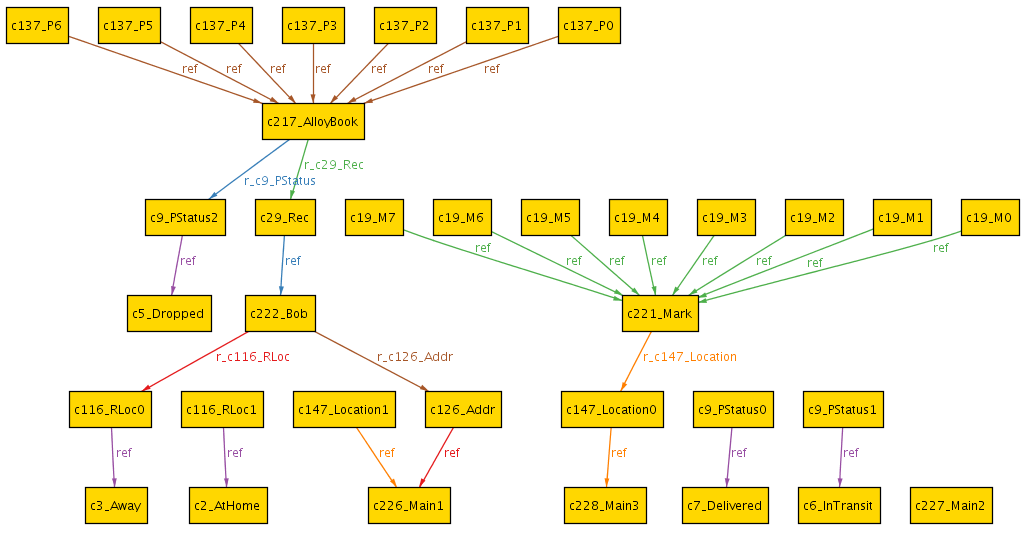
\includegraphics[width=1.1 \textwidth]{Figures/Shipping_Time0.png}
\end{figure}
  \end{frame}

  \begin{frame}
    \frametitle{Parcel service trace (Time=1)}
\begin{figure}
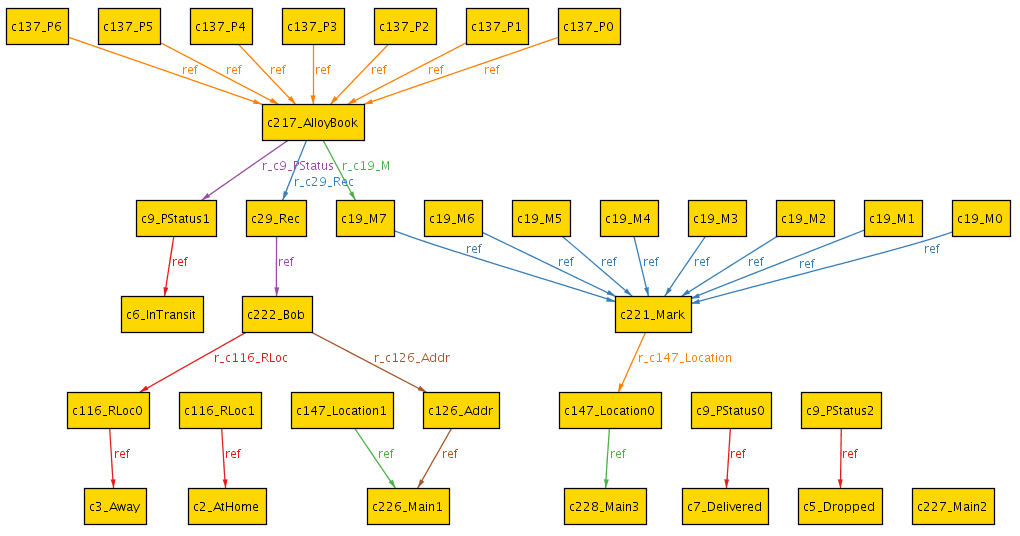
\includegraphics[width=1.1 \textwidth]{Figures/Shipping_Time1.png}
\end{figure}
  \end{frame}
  \begin{frame}
    \frametitle{Parcel service trace (Time=2)}
\begin{figure}
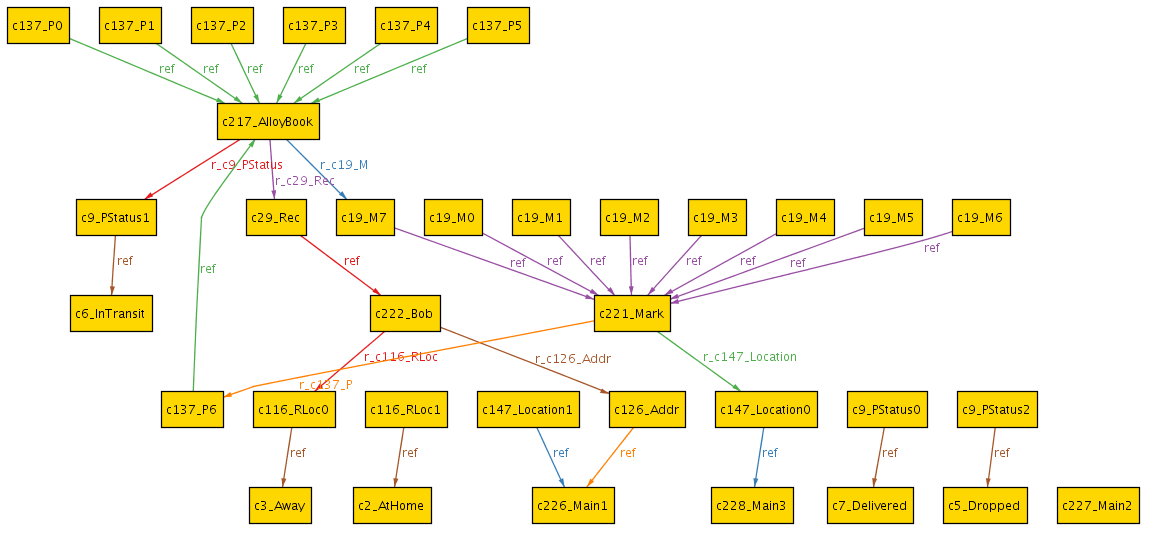
\includegraphics[width=1.1 \textwidth]{Figures/Shipping_Time2.png}
\end{figure}
  \end{frame}
  \begin{frame}
    \frametitle{Parcel service trace (Time=3)}
\begin{figure}
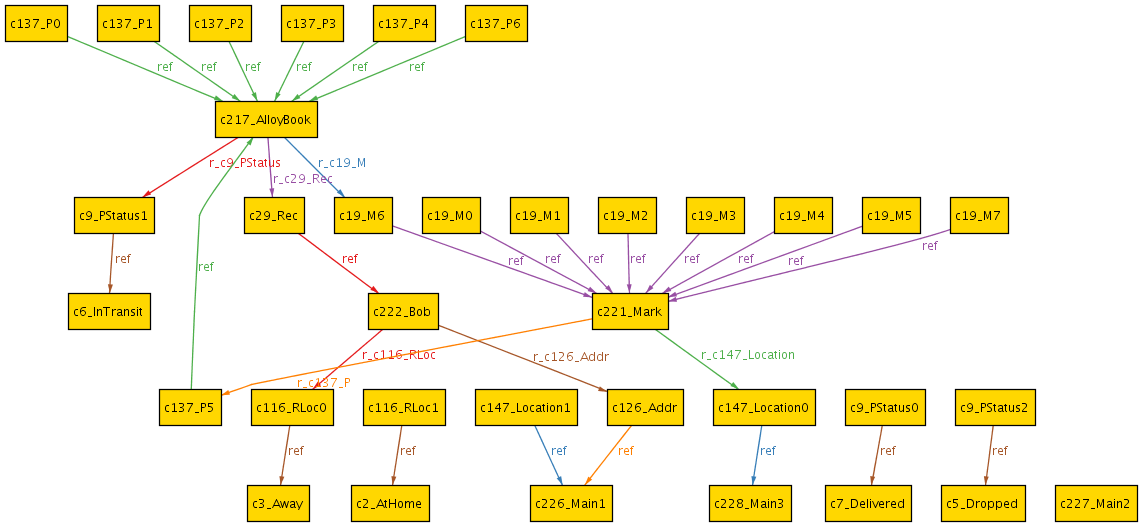
\includegraphics[width=1.1 \textwidth]{Figures/Shipping_Time3.png}
\end{figure}
  \end{frame}
  \begin{frame}
    \frametitle{Parcel service trace (Time=4)}
\begin{figure}
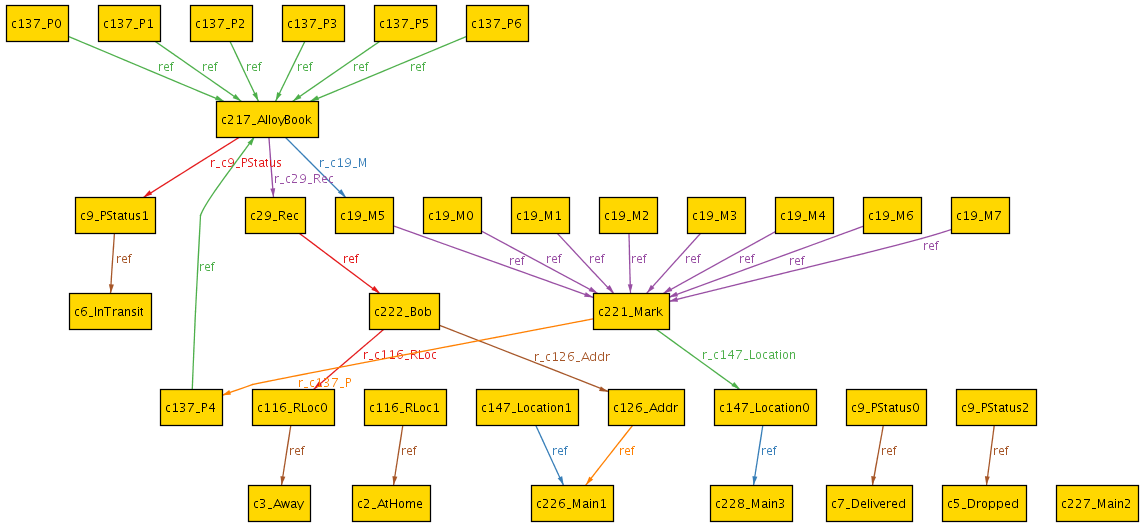
\includegraphics[width=1.1 \textwidth]{Figures/Shipping_Time4.png}
\end{figure}
  \end{frame}
  \begin{frame}
    \frametitle{Parcel service trace (Time=5)}
\begin{figure}
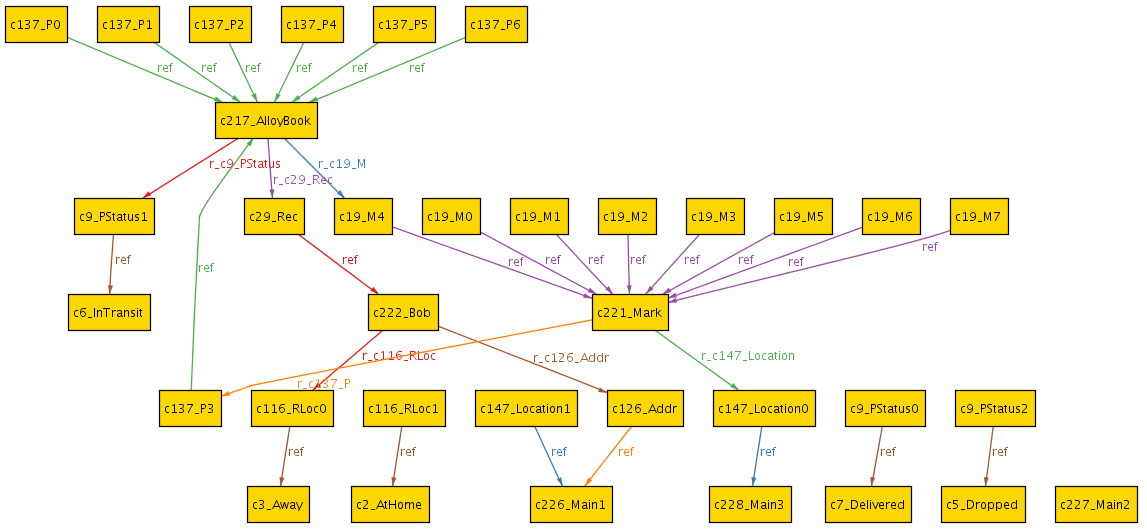
\includegraphics[width=1.1 \textwidth]{Figures/Shipping_Time5.png}
\end{figure}
  \end{frame}
  \begin{frame}
    \frametitle{Parcel service trace (Time=6)}
\begin{figure}
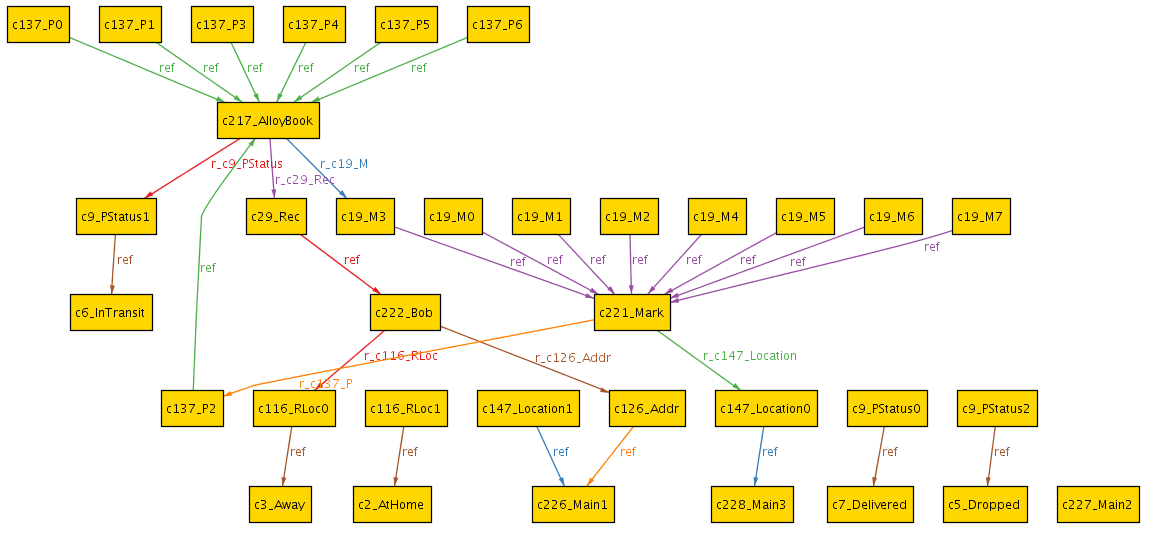
\includegraphics[width=1.1 \textwidth]{Figures/Shipping_Time6.png}
\end{figure}
  \end{frame}
  \begin{frame}
    \frametitle{Parcel service trace (Time=7)}
\begin{figure}
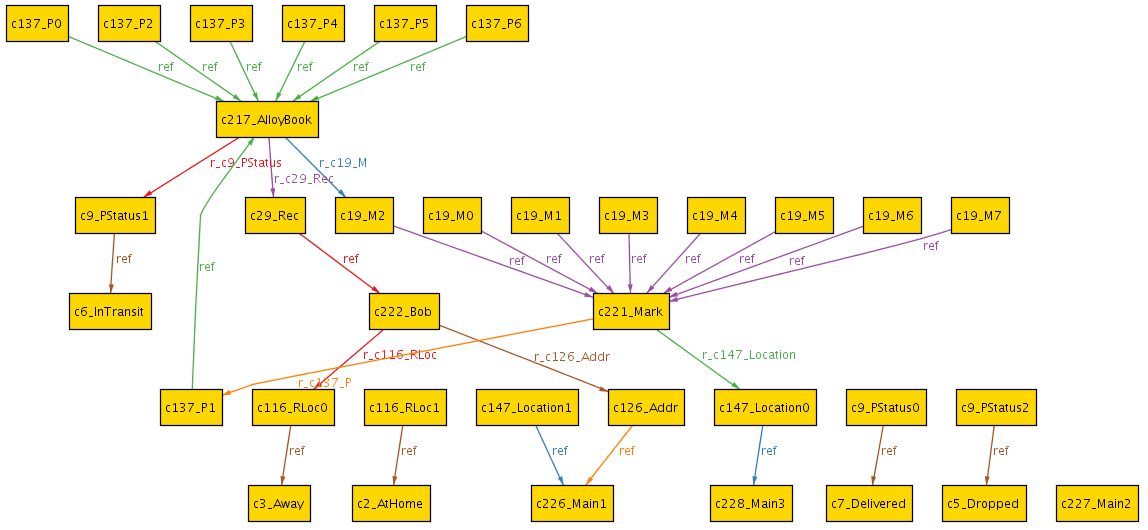
\includegraphics[width=1.1 \textwidth]{Figures/Shipping_Time7.png}
\end{figure}
  \end{frame}
  \begin{frame}
    \frametitle{Parcel service trace (Time=8)}
\begin{figure}
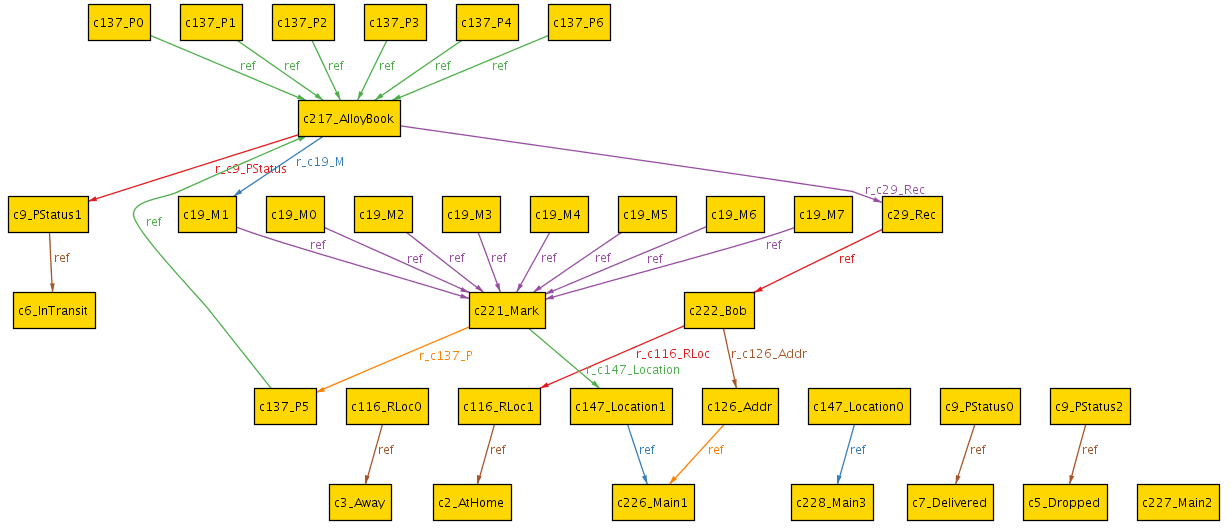
\includegraphics[width=1.1 \textwidth]{Figures/Shipping_Time8.png}
\end{figure}
  \end{frame}
  \begin{frame}
    \frametitle{Parcel service trace (Time=9)}
\begin{figure}
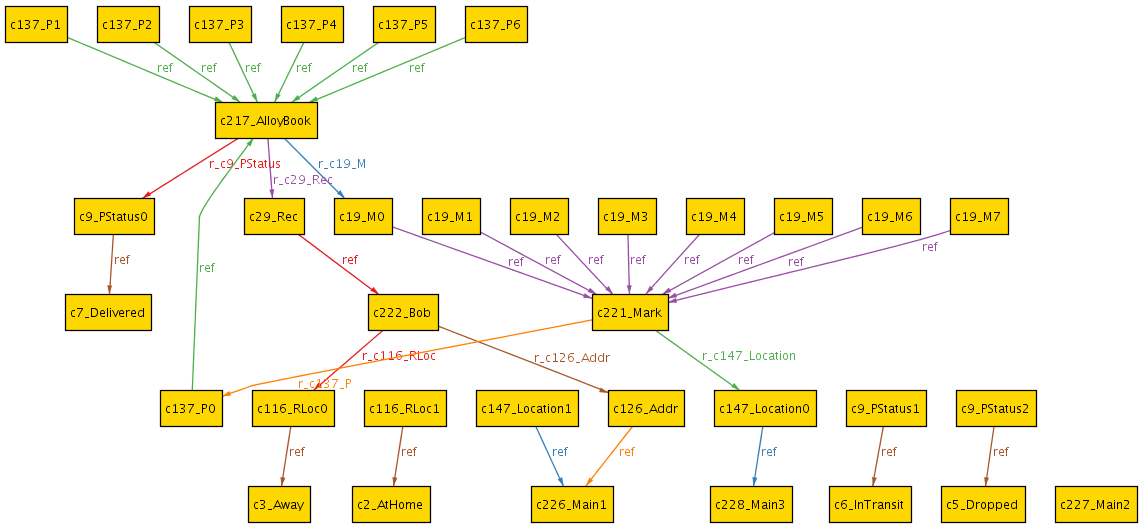
\includegraphics[width=1.1 \textwidth]{Figures/Shipping_Time9.png}
\end{figure}
  \end{frame}

  \begin{frame}
    \frametitle{Open issues/Future work}
    \begin{itemize}
      \item Syntactic solution for referencing current state.
      \item Calculate scope - right now it is just a parameter (--fs=scope).
      \item For reference clafers add Time product to \ttfamily{rel} field instead of appending to field declarations in parent signature. It will prevent generation of unnecessary instances.
      \item Create more models.
    \end{itemize}
  \end{frame}
\end{document}
